\documentclass{beamer}

\usepackage{beamerthemeshadow}
\usepackage{color}
\usepackage{verbatim}
\usepackage{tikz}
\usetikzlibrary{shapes,arrows,positioning,calc}
\usepackage[normalem]{ulem}
\usepackage[timeinterval=10]{tdclock}
%\usepackage{wrapfig}

\mode<presentation>
{
 \usetheme{Warsaw} %%% Change later
\usecolortheme{dove}

%gets rid of bottom navigation bars
%\setbeamertemplate{footline}[page number]{}

% a version with clock in the footline
\setbeamertemplate{footline}
{%
\begin{beamercolorbox}[wd=1.0\paperwidth,ht=2.25ex,dp=1ex,right]{date in head/foot}%
           \usebeamerfont{date in head/foot} \msdark{\insertshortdate{\tdtime}\hspace*{2em}
           \insertframenumber{} / \inserttotalframenumber\hspace*{2ex}} 
        \end{beamercolorbox}%
}

  \setbeamercovered{transparent}
  % or whatever (possibly just delete it)
}


\usepackage{graphicx}

\usepackage{amssymb,soul}

\usepackage{hyperref}

\definecolor{myblue}{rgb}{0, 0, 0.9}

\definecolor{mygreen}{rgb}{0,0.6,0}

\definecolor{mymagenta}{rgb}{0.9, 0, 0.9}

\definecolor{myred}{rgb}{0.9,0,0}

\definecolor{mygray}{rgb}{0.8,0.8,0.8}

\definecolor{mydark}{rgb}{0.4, 0.4, 0.4}

\definecolor{myblack}{rgb}{0,0,0}

\newcommand{\msblue}[1]{{\color{myblue} #1}}

\newcommand{\msmagenta}[1]{{\color{mymagenta} #1}}

\newcommand{\msred}[1]{{\color{myred} #1}}

\newcommand{\msgreen}[1]{{\color{mygreen} #1}}

\newcommand{\msgray}[1]{{\color{mygray} #1}}

\newcommand{\msdark}[1]{{\color{mydark} #1}}

\newcommand{\msblack}[1]{{\color{myblack} #1}}

\newcommand{\relu}{\mbox{\bf ReLU}}

\begin{document}

\title{Exploring synthesis of flexible neural machines with Zygote.jl}
\author{\msmagenta{\bf Mishka (Michael Bukatin)}}
\institute[DMM] % (optional, but mostly needed)
{\href{https://github.com/anhinga}{\tt\small github:anhinga}\\
\ \\
{\small Dataflow Matrix Machines project}
}
\date[]  
{
JuliaCon 2023\\
Cambridge, MA, July 28, 2023}

\begin{frame}
%  \initclock
  \titlepage
\end{frame}

\begin{frame}
  \frametitle{Vectors represented by dictionaries flow through the wires}

\begin{minipage}[t]{0.48\linewidth}
\centering
\begin{tikzpicture}[
  node distance = 1.5cm,
  auto,
  block/.style={
    rectangle,
    draw,
    fill=blue!20,
    text width=5em,
    text centered,
    rounded corners,
    minimum height=4em
  },
  line/.style={draw, -latex'},
  scale=0.35,  % Scale the picture
  transform shape  % Keep the text size the same
]

% Define nodes
\node [block] at (0, 18) (output) {Output};
\node [block] at (6, 15) (compare-5) {compare-5};
\node [block] at (6, 6) (dot-2) {dot-2};
\node [block] at (-3, 12) (compare-4) {compare-4};
\node [block] at (-6, 9) (compare-3) {compare-3};
\node [block] at (-6, 3) (compare-1) {compare-1};
\node [block] at (-3, 6) (norm-2) {norm-2};
\node [block] at (0, 3) (accum-1) {accum-1};
\node [block] at (0, 0) (input) {input};
\node [block] at (6, 0) (eos) {eos};
\node [block] at (-6, 0) (const1) {const1};

% Connect nodes
\path [line] (compare-5) -- node[midway, above, sloped] {true, 1.13} (output);
\path [line] (compare-3) to[out=75,in=-105,looseness=2] node[midway, above, sloped] {false, -1.3} (output);
\path [line] (compare-4) to[out=75,in=-105,looseness=1] node[midway, above, sloped] {false, 1.11} (output);
\path [line] (dot-2) to[out=90,in=-75] node[midway, below, sloped] {-0.71} (compare-5);
\path [line] (dot-2) to[out=90,in=-105] node[midway, below, sloped] {0.7} (compare-5);
\path [line] (norm-2) to[out=90,in=-75] node[midway, below, sloped] {0.64} (compare-4);
\path [line] (norm-2) to[out=90,in=-105] node[midway, above, sloped] {-0.63} (compare-4);
\path [line] (norm-2) to[out=90,in=-75] node[midway, above, sloped] {-0.26} (compare-3);
\path [line] (norm-2) to[out=90,in=-105] node[midway, below, sloped] {0.27} (compare-3);
\path [line] (compare-1) to[out=75,in=-75] node[midway, below, sloped] {false, 0.44} (compare-3);
\path [line] (compare-1) to[out=75,in=-105] node[midway, below, sloped] {false, -0.43} (compare-3);
\path [line] (const1) to[out=90,in=-75] node[midway, below, sloped] {0.43} (compare-1);
\path [line] (const1) to[out=90,in=-105] node[midway, below, sloped] {-0.44} (compare-1);
\path [line] (accum-1) to[out=45,in=-90] node[midway, above, sloped] {0.71} (norm-2);
\path [line] (input) -- node[midway, above, sloped] {0.66} (accum-1);
\path [line] (input) to[out=90,in=-90,looseness=0] node[midway, below, sloped] {-0.46} (norm-2);
\path [line] (eos) -- node[midway, above, sloped] {-1.32} (dot-2);
\path [line] (input) to[out=90,in=210,looseness=0] node[midway, below, sloped] {-0.48} (dot-2);
\path [line] (accum-1) to[out=45,in=210] node[midway, below, sloped] {-0.72} (dot-2);
\path [line, red] (accum-1) to[out=45,in=-45,looseness=5] node[midway, below, sloped, text=red] {1} (accum-1);

\end{tikzpicture}
\end{minipage}
\hfill
\begin{minipage}[t]{0.48\linewidth}
\centering
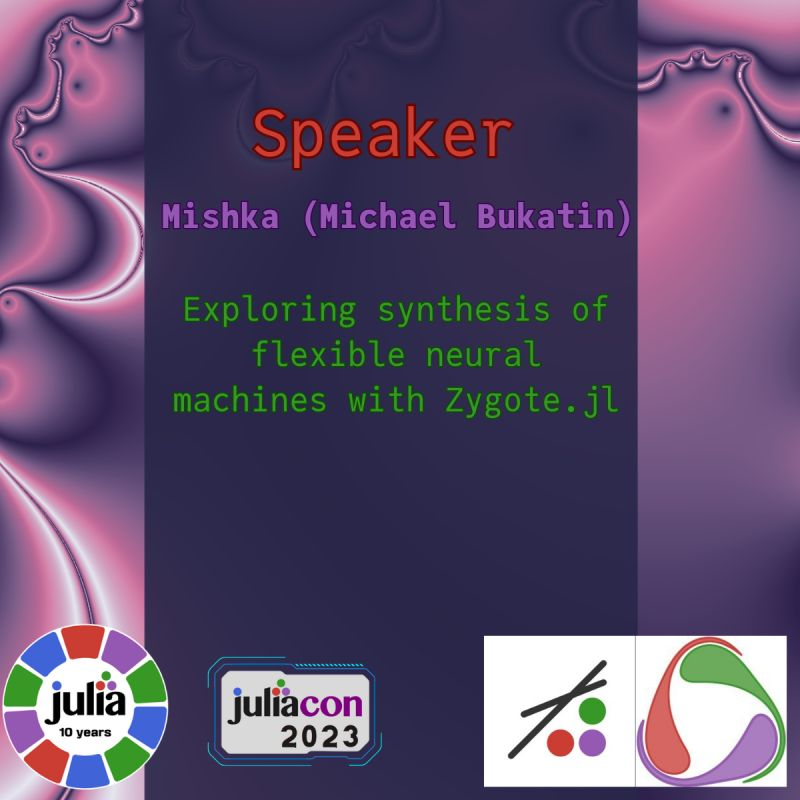
\includegraphics[scale=0.15]{1685638061807}
\end{minipage}

\end{frame}

\begin{frame}

This talk:

\ \\

\begin{itemize}

\item Flexible neural machines (flexible attention machines) discovered and studied by our group a few years ago.\\
        We call them dataflow matrix machines (DMMs).

\ \\

\item My recent experiments with Zygote.jl

\ \\[14ex]

\hspace{2.1in}\msmagenta{I am looking for collaborators}  

\end{itemize}

\end{frame}

\begin{frame}

Transitions:

\ \\

\begin{itemize}

\item Traditional neural nets $\Rightarrow$ \msmagenta{Transformers (modern AI magic)}

\begin{itemize}

\item Much more expressive than traditional neural nets

\item Easier to train (better optimized for training)

\end{itemize}


\ \\

\item Transformers $\Rightarrow$ \msmagenta{Flexible neural machines}

\begin{itemize}

\item Much more expressive than even Transformers

\begin{itemize}
\item General-purpose continuously deformable dataflow programs
\item Convenient and flexible self-modification facilities
\item ...
\end{itemize}

\item But not optimized for training (too flexible)

\begin{itemize}
\item \msmagenta{Zygote.jl is also very flexible and can help today}
\item Optimize those neural machines better in the future?
\end{itemize}

\end{itemize}

\end{itemize}

\end{frame}

\section{Dataflow matrix machines (DMMs)}

\begin{frame}

The essence of neural model of computations is that\\
\msmagenta{linear and non-linear computations are interleaved.}\\[2ex] 

What is the most general (and most flexible) way\\
to make this linear/non-linear alternating pattern possible?\\[2ex]

\dotfill\\[2ex]

The natural degree of generality for neural-like computations is:\\[2ex]
\hspace{0.2in}\sout{use only streams of numbers}\\
\hspace{0.2in}use any streams supporting the notion of\\
\hspace{0.6in}linear combination of several streams \msmagenta{(``linear streams")}

\end{frame}

\begin{frame}

  \frametitle{\msmagenta{Dataflow matrix machines (DMMs)}}

DMMs: a very natural class of {\bf neural machines}.\\[2ex]

They use arbitrary {\bf linear streams} instead of streams of numbers.\\[2ex]

{\bf Use of linear streams by single neurons} is the main source of their power compared to RNNs.
The extra power also comes from:\\[1ex]

\begin{itemize}

\item Arbitrary fixed or variable arity of neurons;\\[2ex]

\item Highly expressive linear streams of V-values\\ (tree-shaped flexible tensors);\\[2ex]

\item Unbounded network size ($\Rightarrow$ unbounded memory);\\[2ex]

\item Self-referential facilities: ability to change weights, topology, and the size of the active part dynamically, on the fly.

\end{itemize}

\end{frame}

\subsection{Linear streams}

\begin{frame}

  \frametitle{\msmagenta{RNNs: linear and non-linear computations are interleaved}}



\begin{columns}[T]
\begin{column}{0.5\textwidth}
\begin{tikzpicture}
   \clip (-2.0, -2.0) rectangle (4.0, 2.0);
   %\draw (-2.0, -2.0) rectangle (4.0, 2.0);
   \draw [->] (-0.8, 0) -- (-0.8, 1) node [left] {$i_m$};
   \draw [->] (-1.6, 0) -- (-1.6, 1) node [left] {$i_1$};
   \filldraw (-1.2,0) circle [radius=0.5pt]
                 (-1.4,0)  circle [radius=0.5pt]
                 (-1.0, 0) circle [radius=0.5pt]
                 (-0.8, 0) circle [radius=1pt]
                 (-1.6, 0) circle [radius=1pt];

 

 \msgreen{  \draw [->] (-0.4, -1) node [left] {\msblack{$x_1$}} -- (-0.4, 1) node [midway, above right] {$f_1$} node [right] {\msblack{$y_1$}};
   \draw [->] (0.4, -1)  node [left] {\msblack{$x_k$}} -- (0.4, 1) node [midway, above right] {$f_k$} node [right] {\msblack{$y_k$}};}
   \filldraw (0,0) circle [radius=0.5pt]
                 (-0.2,0)  circle [radius=0.5pt]
                 (0.2, 0) circle [radius=0.5pt];

   \draw (0.8, -1) node [right] {$o_1$} -- (0.8, 0);
   \draw (1.6, -1) node [right] {$o_n$} -- (1.6, 0);
   \filldraw (1.2,0) circle [radius=0.5pt]
                 (1.4,0)  circle [radius=0.5pt]
                 (1.0, 0) circle [radius=0.5pt]
                 (0.8, 0) circle [radius=1pt]
                 (1.6, 0) circle [radius=1pt]; 

\msblue{\draw [->, very thick] (0, 1.2) .. controls (3.5, 4.2) and (3.5, -4.2) .. (0, -1.2)  node [midway, right] {{\bf W}};}

\end{tikzpicture}

\end{column}
\begin{column}{0.5\textwidth}

``Two-stroke engine" for an RNN:\\[3ex]


``Down movement" \msblue{(linear$^1$)}:\\[2ex] 

$(x_1^{t+1}, \ldots, x_k^{t+1}, o_1^{t+1}, \ldots, o_n^{t+1})^{\top}=$\\[0.1ex] \msblue{{\bf W}}$ \cdot (y_1^{t}, \ldots, y_k^{t}, i_1^{t}, \ldots, i_m^{t})^{\top}$.\\[3ex]

``Up movement" \msgreen{(non-linear$^2$)}:\\[2ex]  

$y_1^{t+1} = \msgreen{f_1}(x_1^{t+1}), \ldots,$\\[0.1ex]$y_k^{t+1} = \msgreen{f_k}(x_k^{t+1})$.

\end{column}
\end{columns}

\hrulefill

\msblue{\footnotesize $^1$ linear and global in terms of connectivity}\\
\msgreen{\footnotesize $^2$ usually non-linear, local}

\end{frame}


\begin{frame}

\frametitle{\msmagenta{Linear streams}}

The key feature of {\bf DMMs} compared to {\bf RNNs}:
         they use\\ {\bf linear streams} instead of streams of numbers.\\[2ex]

The following streams all support the pattern of alternating\\ linear and non-linear computations:\\[2ex]

\begin{itemize}

\item Streams of numbers\\[2ex]

\item Streams of vectors from fixed vector space $V$\\[2ex]

\item Linear streams: such streams that the notion of\\ {\bf linear combination of several streams} is defined.\\[3ex]

\end{itemize}

\msmagenta{{\bf ``Artificial attention"}:\\ taking linear combinations of high-dimensional objects.}






\end{frame}




\begin{frame}

\frametitle{Kinds of linear streams}

\msmagenta{The notion of {\bf linear streams} is more general than the notion
of {\bf streams of vectors}.} Some examples:\\[1ex]


\begin{itemize}


\item Every vector space $V$ gives rise to the corresponding kind of linear streams
(streams of vectors from that space)\\[2ex]

\item \msmagenta{Every measurable space $X$ gives rise to the space of\\ {\bf streams of
probabilistic samples} drawn from $X$\\ and decorated with +/- signs\\
(linear combination is defined by a stochastic procedure)}\\[2ex]

\item Streams of images of a particular size (that is, animations)\\[2ex]

\item Streams of matrices; streams of multidimensional arrays\\[2ex]

\item Streams of V-values based on nested maps (\msmagenta{trees})\\[2ex]



\end{itemize}

\end{frame}








\begin{frame}

  \frametitle{\msmagenta{Dataflow matrix machines  (DMMs, continued)}}

Countable network with finite active part at any moment of time.\\[2ex]

Countable matrix \msblue{{\bf W}} with finite number of non-zero elements at any moment of time.

\begin{columns}[T]
\begin{column}{0.7\textwidth}
\begin{tikzpicture}
   \clip (-3.0, -2.0) rectangle (5.0, 2.0);
   %\draw (-2.0, -2.0) rectangle (4.0, 2.0);
  \filldraw (-3.2,0) circle [radius=0.5pt]
                (-3.0,0)  circle [radius=0.5pt]
                (-3.4, 0) circle [radius=0.5pt]; 

\msgreen{   \draw [->] (-1.2, 0) -- (-0.8, 1) node [right] {\msblack{$y_{2,C_1}$}};
   \draw [->] (-1.2, 0) -- (-1.6, 1) node [left] {\msblack{$y_{1,C_1}$}};
   \draw (-2.0, -1)  node [left] {\msblack{$x_{1,C_1}$}} -- (-1.2, 0);
   \draw (-1.2, -1)  node [below] {\msblack{$x_{2,C_1}$}} -- (-1.2, 0) node [left] {$f_{C_1}$};
   \draw (-0.4, -1)  node [right] {\msblack{$x_{3,C_1}$}} -- (-1.2, 0);}


  \filldraw (0,0) circle [radius=0.5pt]
                (-0.2,0)  circle [radius=0.5pt]
                (0.2, 0) circle [radius=0.5pt];


 \msgreen{    \draw (1.6, -1) node [left] {\msblack{$x_{1,C_2}$}} -- (2.0, 0)  node [left] {$f_{C_2}$};;
   \draw (2.4, -1) node [right] {\msblack{$x_{2,C_2}$}} -- (2.0, 0);
   \draw [->] (2.0, 0) -- (1.2, 1) node [left] {\msblack{$y_{1,C_2}$}};
   \draw [->] (2.0, 0) -- (2.0, 1) node [above] {\msblack{$y_{2,C_2}$}};
   \draw [->] (2.0, 0) -- (2.8, 1) node [right] {\msblack{$y_{3,C_2}$}};}


  \filldraw (3.2,0) circle [radius=0.5pt]
                (3.0,0)  circle [radius=0.5pt]
                (3.4, 0) circle [radius=0.5pt]; 


  \msblue{\draw [->, very thick] (0.5, 1.2) .. controls (5.5, 4.2) and (5.5, -4.2) .. (0.5, -1.2)  node [midway, right] {{\bf W}};}

\end{tikzpicture}

\end{column}
\begin{column}{0.3\textwidth}

{%\scriptsize
\tiny
``Down movement": 

\msblue{For all inputs $x_{i,C_k}$ where there is a non-zero weight $w_{(i,C_k), (j,C_m)}^t$:}\\[1ex]

{\scriptsize$x_{i,C_k}^{t+1} = \msblue{\sum}_{\{(j,C_m) | w_{(i,C_k), (j,C_m)}^t \neq 0\}}$\\[0.1ex]$\msblue{w_{(i,C_k), (j,C_m)}^t }* y_{j, C_m}^{t}.$}\\[3ex]

``Up movement":\\[0.1ex]  

\msgreen{For all active neurons $C$:}\\[1ex]

{\scriptsize $y^{t+1}_{1,C},...,y^{t+1}_{p,C} = \msgreen{f_C} (x^{t+1}_{1,C},...,x^{t+1}_{n,C})$.}
}

\end{column}
\end{columns}


Here $x_{i,C_k}$ and $y_{j,C_m}$ are linear streams.\\
\msmagenta{Neurons in DMMs have arbitrary arity!}

\end{frame}







\section{V-values and variadic neurons}







\begin{frame}

  \frametitle{Type correctness condition  for mixing different kinds of linear streams in one DMM}


\msmagenta{Type correctness condition:} $w_{(i,C_k), (j,C_m)}^t$ is allowed to be
non-zero only if $x_{i,C_k}$ and $y_{j, C_m}$ belong to the same {\bf kind} of linear streams.\\[6ex]

{\bf Next:} \msmagenta{linear streams of {\bf V-values} based on {\bf nested dictionaries}:}\\[2ex]

\begin{itemize}

\item sufficiently universal and expressive to save us from the need to impose type correctness conditions.\\[2ex]

\item allow us to define {\bf variadic neurons}, so that we don't need to keep track of input and output
arity either.
\end{itemize}

\end{frame}








\subsection{Vectors based on nested maps}


\begin{frame}

  \frametitle{\msmagenta{V-values: vector space based on nested dictionaries}}


V-values play the role of Lisp S-expressions in this formalism.\\[3ex]


We want a vector space.\\[3ex]

Take prefix trees with numerical leaves\\ implemented as nested dictionaries.\\[3ex]

We call them {\bf V-values}
(``vector-like values").\\[3ex]

\hrulefill

(A more general construction of V-values with ``linear stream" leaves:  Section 5.3 of \href{https://arxiv.org/abs/1712.07447}{\tt\footnotesize  https://arxiv.org/abs/1712.07447})

\end{frame}





\begin{frame}

  \frametitle{\msmagenta{Ways to understand V-values}}

Consider ordinary words (``labels") to be letters of a countable ``super-alphabet" $L$.\\[2ex]

V-values can be understood as

\begin{itemize}

  \item Finite linear combinations of finite strings of letters from $L$;
  \item Finite prefix trees with numerical leaves;
  \item Sparse ``tensors of mixed rank" with finite number of non-zero elements;
  \item Recurrent maps (that is, nested dictionaries) from $V \cong \mathbb{R}\oplus (L \rightarrow V)$  admitting finite descriptions.

\end{itemize}

\end{frame}


\begin{frame}

  \frametitle{\msmagenta{Example of a V-value: different ways to view it}}

\begin{columns}[T]
\begin{column}{0.5\textwidth}

\begin{tikzpicture}
  \clip (-3.0, -4.5) rectangle (3.0, 0.0);

  \draw[->](0, 0) -- (-1.8, -1)  node [below] {3.5};

  \draw[->](0, 0) -- (0, -1) node [midway,  below right] {:foo};

    \draw[->](0, -1) -- (0.5, -2) node[midway, below right] {\ :bar};

      \draw[->](0.5, -2) -- (0.5, -3) node [below] {7};

    \draw[->](0, -1) -- (-0.5, -2) node [below] {2};

  \draw[->](0, 0) -- (1.8, -1) node [midway, below  right] {\ \ \ \ \ \ :baz};

      \draw[->](1.8, -1) -- (1.8, -2) node [midway, below  right] {:foo};

      \draw[->](1.8, -2) -- (1.8, -3) node [midway, below  right] {:bar};      

      \draw[->](1.8, -3) -- (1.8, -4) node [below] {-4};
 

  \filldraw (1.8, -1) circle [radius=0.7pt]
                (1.8, -2) circle [radius=0.7pt]
                (1.8, -3) circle [radius=0.7pt]
                (0, -1) circle [radius=0.7pt]
                (0.5, -2) circle [radius=0.7pt];
  
 

\end{tikzpicture}
\end{column}
\begin{column}{0.5\textwidth}

\begin{itemize}

{\footnotesize

 \item 3.5 $\cdot$ ($\epsilon$) + 2 $\cdot$ (:foo) + \\ 7 $\cdot$ (:foo :bar) - 4 $\cdot$ (:baz :foo :bar)

 \item ($\leadsto$ 3.5) + (:foo $\leadsto$  2) +\\ (:foo $\leadsto$ :bar $\leadsto$ 7) +\\
          (:baz $\leadsto$ :foo $\leadsto$ :bar $\leadsto$ -4)


\msmagenta{
 \item {\tiny  scalar 3.5 + sparse 1D array \{{\tt d1[:foo]= 2}\} +\\[1.5ex] sparse 2D
matrix \{{\tt d2[:foo, :bar]= 7}\} +\\  sparse 3D array \{{\tt d3[:baz, :foo, :bar]= -4}\}}
}

 \item {\tt \{:number 3.5,\\ :foo \{:number 2, :bar 7\}, :baz \{:foo \{:bar -4\}\}\}}
          ({\tt :number} $\not\in L$)

}

\end{itemize}

\end{column}
\end{columns}

\end{frame}






\subsection{Variable arity}


\begin{frame}

  \frametitle{Dataflow matrix machines (DMMs) based on\\
 streams of  V-values
 and
 variadic neurons}

$x_{f, n_f, i}^{t+1} = \sum_{g \in F} \sum_{n_g \in L} \sum_{o \in L} \msblue{w_{f, n_f, i;\, g, n_g, o}^t} * y_{g, n_g, o}^t$ {\small \msblue{(down movement)}}\\[2ex]

$y_{f, n_f}^{t+1} = f(x_{f, n_f}^{t+1})$ {\small \msgreen{(up movement)}}

\begin{tikzpicture}
  %\draw (-3.5, -2.0) rectangle (7.0, 2.0);
  \clip (-3.5, -2.0) rectangle (7.0, 2.0);

  \filldraw (-3.2,0) circle [radius=0.5pt]
                (-3.0,0)  circle [radius=0.5pt]
                (-3.4, 0) circle [radius=0.5pt]; 

\msgreen{\draw [->] (-2.6, -1.5) node[right] {\msmagenta{$x_{f, n_f}$}} -- (-2.6, 1.5) node [midway, above right] {$f$} node[right] {\msmagenta{$y_{f, n_f}$}};}

  \filldraw (0,0) circle [radius=0.5pt]
                (-0.2,0)  circle [radius=0.5pt]
                (0.2, 0) circle [radius=0.5pt];

\msgreen{\draw [->] (0.6, -1.5) node[right] {\msmagenta{$x_{g, n_g}$}} -- (0.6, 1.5) node [midway, above right] {$g$} node[right] {\msmagenta{$y_{g, n_g}$}};}

  \filldraw (3.2,0) circle [radius=0.5pt]
                (3.0,0)  circle [radius=0.5pt]
                (3.4, 0) circle [radius=0.5pt]; 


 \msblue{ \draw [->, very thick] (1.1, 1.1) .. controls (5.5, 4.3) and (5.5, -4.0) .. (1.1, -0.8)  node [midway, right] {{\bf W}};}

  \foreach \y in {-1.0, 1.0}
    {

      \draw [densely dotted] (0.45, \y+0.15) ellipse [x radius=100pt, y radius=4pt];

     \foreach \x in {-1.0, 2.2}
       {

        \foreach \d in {-0.4, -0.15, 0.1}
           {
               \msmagenta{\draw(\x-0.15, \y + 0.45) -- (\x+\d, \y+0.15); 
               \draw (\x+\d, \y + 0.15) -- (\x+\d-0.08, \y-0.15);
               \draw (\x+\d, \y + 0.15) -- (\x+\d+0.08, \y-0.15);
               \filldraw (\x+0.5*\d-0.05, \y-0.25) circle [radius=0.2pt];
               \filldraw (\x+0.5*\d+0.5, \y+0.15) circle [radius=0.2pt];}
           }
       } 
     }
 
\end{tikzpicture}

\end{frame}

\section{Programming patterns and self-referential facilities}




\begin{frame}

  \frametitle{\msmagenta{DMMs: programming with powerful neurons}}

Powerful variadic neurons and streams of V-values $\Rightarrow$ a much more expressive formalism
 than networks based on streams of numbers.\\[2ex]

$\Rightarrow$ Many tasks can be accomplished by \msmagenta{compact DMM networks},\\
 where {\bf single neurons function as layers or modules}.

\hrulefill

\begin{itemize}

\item \msmagenta{Accumulators and memory}

\item Multiplicative constructions and ``fuzzy if"

\item \msmagenta{Sparse vectors}

\item Data structures

\item Self-referential facilities

\end{itemize}






\end{frame}

\begin{frame}

  \frametitle{\msmagenta{Accumulators and memory}}

\begin{tikzpicture}
   \clip (-2.0, -2.0) rectangle (7.0, 2.0);




  \filldraw (0,0) circle [radius=0.5pt]
                (-0.2,0)  circle [radius=0.5pt]
                (0.2, 0) circle [radius=0.5pt];

\msgreen{\draw [->] (0.6, -1.5) node[right] {\msblack{$x_{{\tt plus}, {\tt :my\mbox{\footnotesize -}neuron}}$}} -- 
                    (0.6, 1.5) node [midway, above right] {\tt plus} node[right]
                    {\msblack{$y_{{\tt plus}, {\tt :my\mbox{\footnotesize -}neuron}}$}};}

  \filldraw (3.2,0) circle [radius=0.5pt]
                (3.0,0)  circle [radius=0.5pt]
                (3.4, 0) circle [radius=0.5pt]; 


 \msblue{\draw [->] (1.9, 1.1) .. controls (5.5, 4.3) and (5.5, -4.0) .. (2.15, -0.85)  node [midway, left] {{1.0}};

  \draw [->] (1.7, -0.2) -- (1.5, -0.9);
  \filldraw (1.5, -0.25) circle [radius=0.2pt];
  \filldraw (1.6, -0.25) circle [radius=0.2pt];
  \filldraw (1.4, -0.25) circle [radius=0.2pt];
  \draw [->] (1.3, -0.2) node [left] {{\tiny updates from other neurons}} -- (1.5, -0.8);}


  \foreach \y in {-1.0}
    {

      \draw [densely dotted] (1.0, \y+0.15) ellipse [x radius=80pt, y radius=5pt];

     \foreach \x in {2.0}
       {

        \foreach \d in {-0.4}
           {
               \draw(\x-0.15, \y + 0.45) -- (\x+\d, \y+0.15) node [left] {\scriptsize{\tt :delta}}; 
               \draw (\x+\d, \y + 0.15) -- (\x+\d-0.08, \y-0.15);
               \draw (\x+\d, \y + 0.15) -- (\x+\d+0.08, \y-0.15);
               \filldraw (\x+0.5*\d-0.05, \y-0.25) circle [radius=0.2pt];
               %\filldraw (\x+0.5*\d+0.5, \y+0.15) circle [radius=0.2pt];
           }
       \foreach \d in {0.1}
           {
               \draw(\x-0.15, \y + 0.45) -- (\x+\d, \y+0.15) node [right] {\scriptsize{\tt :accum}}; 
               \draw (\x+\d, \y + 0.15) -- (\x+\d-0.08, \y-0.15);
               \draw (\x+\d, \y + 0.15) -- (\x+\d+0.08, \y-0.15);
               \filldraw (\x+0.5*\d-0.05, \y-0.25) circle [radius=0.2pt];
               %\filldraw (\x+0.5*\d+0.5, \y+0.15) circle [radius=0.2pt];
           }
        \foreach \d in {-0.4, -0.15, 0.1}
           {
              \filldraw (\x+0.5*\d-0.05, \y-0.25) circle [radius=0.2pt];
           }
       } 
     }

  \foreach \y in {0.9}
    {

      \draw [densely dotted] (1.0, \y+0.15) ellipse [x radius=80pt, y radius=5pt];

     \foreach \x in {2.0}
       {

        \foreach \d in {-0.15}
           {
               \draw(\x-0.15, \y + 0.45) -- (\x+\d, \y+0.15) node [right] {\scriptsize{\tt :single}}; 
               \draw (\x+\d, \y + 0.15) -- (\x+\d-0.08, \y-0.15);
               \draw (\x+\d, \y + 0.15) -- (\x+\d+0.08, \y-0.15);
 
               %\filldraw (\x+0.5*\d+0.5, \y+0.15) circle [radius=0.2pt];
           }
        \foreach \d in {-0.4, -0.15, 0.1}
           {
              \filldraw (\x+0.5*\d-0.05, \y-0.25) circle [radius=0.2pt];
           }
       } 
     }
 
\end{tikzpicture}

In this implementation, activation function \msgreen{\footnotesize \tt plus} adds V-values from 
{\footnotesize\tt :accum} and {\footnotesize\tt :delta}
together and places the result into {\footnotesize\tt :single}.

\end{frame}

\begin{frame}

  \frametitle{Multiplicative masks and fuzzy conditionals (gating)}

\msmagenta{Many multiplicative constructions enabled by {\bf input arity $>1$}.}\\[2ex]

The most notable is multiplication of an otherwise computed
neuron output by the value of one of its scalar inputs.\\[2ex]

This is essentially a {\bf fuzzy conditional}, which can
\begin{itemize} 
\item selectively
turn parts of the network on and off in real time\\ via multiplication by zero
\item attenuate or amplify the signal
\item  reverse the signal
via multiplication by -1
\item  redirect
flow of signals in the network
\item ... \\[2ex]
\end{itemize}

\end{frame}


\subsection{Sparse vectors}



\begin{frame}

  \frametitle{\msmagenta{Sparse vectors of high or infinite dimension}}

Example:  a neuron accumulating count of words in a given text.\\[2ex]

The dictionary mapping words to their respective counts is an infinite-dimensional vector
with a finite number of non-zero elements.\\[2ex]

\msmagenta{\Large $\bullet$} Don't need a neuron for each coordinate of our vector space.\\[2ex]

 \msmagenta{\Large $\bullet$} Don't have an obligation to reduce dimension by embedding.

\end{frame}





\subsection{Data structures}





\begin{frame}

  \frametitle{Streams of immutable \msmagenta{data structures}}

One can represent {\bf lists, matrices, graphs,} and so on\\ via nested dictionaries.\\[3ex]


It is natural to use streams of immutable V-values in the implementations of DMMs.\\[3ex]

The DMM architecture is friendly towards algorithms working with immutable data structures in
the spirit of functional programming.\\[3ex]

But more imperative styles can be accommodated as well.

\end{frame}





\subsection{Self-referential facilities}

\begin{frame}

  \frametitle{\msmagenta{Self-referential facilities}}

Difficult to do well with streams of scalars because of dimension mismatch:
typically one has $\sim N$ neurons and $\sim N^2$ weights.\\[2ex]

\msmagenta{Easy in DMMs:}\\[2ex]

It is easy to represent the network matrix {\bf W} as a V-value.\\[2ex]

Emit the stream
of network matrices from neuron {\tt Self}.\\[2ex]

Use the most recent V-value from that stream
as the network matrix {\bf W} during the
next ``down movement".\\[2ex]

This mechanism allows a DMM network to 
{\bf modify its own weights, topology, and size}
while it is running.

\end{frame}


\begin{frame}

  \frametitle{\msmagenta{Self-referential facilities}}

Our current implementation: {\tt Self} connected as an accumulator.\\[2ex]
It accumulates the value of the network matrix and
accepts additive updates from other neurons in the network.\\[2ex]

\begin{tikzpicture}
   \clip (-2.0, -2.0) rectangle (7.0, 2.0);




  \filldraw (0,0) circle [radius=0.5pt]
                (-0.2,0)  circle [radius=0.5pt]
                (0.2, 0) circle [radius=0.5pt];

  \msgreen{\draw [->] (0.6, -1.5) node[right] {\msblack{$x_{{\tt plus}, {\bf :Self}}$}} -- 
                    (0.6, 1.5) node [midway, above right] {{\tt plus}} node[right] {\msblack{$y_{{\tt plus}, {\bf :Self}}$}};}

  \filldraw (3.2,0) circle [radius=0.5pt]
                (3.0,0)  circle [radius=0.5pt]
                (3.4, 0) circle [radius=0.5pt]; 


  \msblue{\draw [->] (1.9, 1.1) .. controls (5.5, 4.3) and (5.5, -4.0) .. (2.15, -0.85)  node [midway, left] {{1.0}};

  \draw [->] (1.7, -0.2) -- (1.5, -0.9);
  \filldraw (1.5, -0.25) circle [radius=0.2pt];
  \filldraw (1.6, -0.25) circle [radius=0.2pt];
  \filldraw (1.4, -0.25) circle [radius=0.2pt];
  \draw [->] (1.3, -0.2) node [left] {{\tiny updates from other neurons}} -- (1.5, -0.8);}


  \foreach \y in {-1.0}
    {

      \draw [densely dotted] (1.0, \y+0.15) ellipse [x radius=80pt, y radius=5pt];

     \foreach \x in {2.0}
       {

        \foreach \d in {-0.4}
           {
               \draw(\x-0.15, \y + 0.45) -- (\x+\d, \y+0.15) node [left] {\scriptsize{\tt :delta}}; 
               \draw (\x+\d, \y + 0.15) -- (\x+\d-0.08, \y-0.15);
               \draw (\x+\d, \y + 0.15) -- (\x+\d+0.08, \y-0.15);
               \filldraw (\x+0.5*\d-0.05, \y-0.25) circle [radius=0.2pt];
               %\filldraw (\x+0.5*\d+0.5, \y+0.15) circle [radius=0.2pt];
           }
       \foreach \d in {0.1}
           {
               \draw(\x-0.15, \y + 0.45) -- (\x+\d, \y+0.15) node [right] {\scriptsize{\tt :accum}}; 
               \draw (\x+\d, \y + 0.15) -- (\x+\d-0.08, \y-0.15);
               \draw (\x+\d, \y + 0.15) -- (\x+\d+0.08, \y-0.15);
               \filldraw (\x+0.5*\d-0.05, \y-0.25) circle [radius=0.2pt];
               %\filldraw (\x+0.5*\d+0.5, \y+0.15) circle [radius=0.2pt];
           }
        \foreach \d in {-0.4, -0.15, 0.1}
           {
              \filldraw (\x+0.5*\d-0.05, \y-0.25) circle [radius=0.2pt];
           }
       } 
     }

  \foreach \y in {0.9}
    {

      \draw [densely dotted] (1.0, \y+0.15) ellipse [x radius=80pt, y radius=5pt];

     \foreach \x in {2.0}
       {

        \foreach \d in {-0.15}
           {
               \draw(\x-0.15, \y + 0.45) -- (\x+\d, \y+0.15) node [right] {\scriptsize{\bf :NetworkMatrix}}; 
               \draw (\x+\d, \y + 0.15) -- (\x+\d-0.08, \y-0.15);
               \draw (\x+\d, \y + 0.15) -- (\x+\d+0.08, \y-0.15);
 
               %\filldraw (\x+0.5*\d+0.5, \y+0.15) circle [radius=0.2pt];
           }
        \foreach \d in {-0.4, -0.15, 0.1}
           {
              \filldraw (\x+0.5*\d-0.05, \y-0.25) circle [radius=0.2pt];
           }
       } 
     }
 
\end{tikzpicture}

The most recent V-value at the {\footnotesize\tt :NetworkMatrix} output of\\ $y_{{\tt plus}, {\bf :Self}}$ neuron is used as \msblue{\bf W}.


\end{frame}


\begin{frame}

  \frametitle{Self-referential facilities}


Other neurons can use {\tt Self} outputs to take into account
the structure and weights of the current network {\bf (reflection)}.\\[2ex]

We have used self-referential mechanism to obtain waves of connectivity
patterns propagating within the network matrix.\\[2ex]

We have observed
interesting self-organizing patterns in self-referential networks.\\[2ex]

We also use this mechanism for ``pedestrian purposes":\\ to allow
a user to edit a running network on the fly.\\[4ex]

\hspace{2.1in}\msmagenta{AI safety issues are quite real here} 

\end{frame}


\section{Zygote.jl and DMMs}

\begin{frame}

  \frametitle{Promise of DMMs}

\begin{itemize} 

\item \msmagenta{{\bf Learning to learn}}\\[2ex]

We expect that networks which modify themselves should be able to {\bf learn to modify themselves better}.\\[2ex]

\item \msmagenta{{\bf Program synthesis}}\\[2ex]

DMMs combine\\

\begin{itemize}

\item aspects of {\bf program synthesis} setup\\ (compact, human-readable programs);\\

\item aspects of {\bf program inference} setup\\ (continuous models defined by matrices).\\[2ex]

\end{itemize} 

\item \msmagenta{{\bf But how to turn this promise into reality?}}
\end{itemize}

\end{frame}

\begin{frame}

  \frametitle{Julia Flux and Zygote.jl}

Julia Flux/Zygote.jl is the first machine learning system with enough flexibility to
work with flexible DMMs and V-values ``as is".\\[4ex]

In particular, this has been the first machine learning system which can take 
{\bf gradients with respect to trees}.\\[4ex]

There is some competition now (e.g. JAX, Enzyme.jl), but Zygote.jl remains my favorite so far.

\end{frame}


\subsection{Synthesis of flexible neural machines}

\begin{frame}

  \frametitle{Neural architecture search}

We use neural architecture search to synthesize a neural machine with desired properties:\\[2ex]

Consider a neural machine consisting of modules (DMM neurons) 
connected with data pipelines gated by scalars (DMM weights).\\[2ex]

\begin{tikzpicture}

  % Define the two rectangles
  \node[draw, rectangle, minimum width=2cm, minimum height=1.5cm] (R1) at (0,0) {};
  \node[draw, rectangle, minimum width=2cm, minimum height=1.5cm] (R2) at (4,0) {};

  % Draw the fat arrow
  \draw[->, line width=2pt] (R1) -- (R2);

  % Draw the thin arrow above the fat arrow
  \draw[->, line width=1pt] ([yshift=0.3cm]R1.east) -- ([yshift=0.3cm]R2.west);

  % Draw alpha over the thin arrow
  \node at (2,0.5) {$\alpha$};

\end{tikzpicture}

{\bf\small Data in the pipeline are multiplied by the scalar $\alpha$}\\[2ex]

Take a large network with modules connected with each other in this fashion and start training it
with {\em sparsifying regularization}, and at some point start {\bf gradually pruning} those connections
which have small $\alpha$ while continuing to train.


\end{frame}

\begin{frame}

  \frametitle{DMM synthesis via neural architecture search}

In our case, modules are DMM neurons, data pipelines carry\\ linear streams of dictionaries,
and $\alpha$ are DMM weights.\\[2ex]

I am going to synthesize a feedforward DMM.\\[2ex]

Let's take a feedforward network with fully connected layers, and with skip connections,
so that each layer is fully connected to each subsequent layer (before we start pruning).\\[2ex]

\begin{tikzpicture}[
    >=stealth,
    neuron/.style={circle, draw, minimum size=0.1cm},
    smalldot/.style={circle, fill, minimum size=0.2cm, inner sep=0pt}
]

% Draw the neurons
\foreach \m/\l [count=\y] in {1,2,3}
  \node [neuron] (input-\m) at (0,2.5-\y) {};

\foreach \m/\l [count=\y] in {1,2,3}
  \node [neuron] (hidden-\m) at (3,3.0-1.3*\y) {};

\foreach \m/\l [count=\y] in {1,2,3}
\node [smalldot] (output-\m) at (5,3.0-1.3*\y) {};

\foreach \m/\l [count=\y] in {1,2,3}
  \node [neuron] (output-\m) at (7,2.5-\y) {};

% Connect every node in the input layer with every node in the
% hidden layer and every node in the output layer
\foreach \i in {1,2,3}
  \foreach \j in {1,2,3}
    \draw [->] (input-\i) -- (hidden-\j);

\foreach \i in {1,2,3}
  \foreach \j in {1,2,3}
    \draw [->, blue] (input-\i) -- (output-\j);


\end{tikzpicture}

\end{frame}

\begin{frame}

  \frametitle{A handcrafted DMM implementing a duplicate detector}

\begin{tikzpicture}[
    node distance = 2cm,
    auto,
    thick,
    block/.style = {
        rectangle,
        draw,
        fill=blue!20,
        text width=5em,
        text centered,
        rounded corners,
        minimum height=4em
    },
    line/.style = {
        draw,
        -latex'
    },
   scale=0.5,  % Scale the picture
   transform shape  % Keep the text size the same
]

    % Define nodes
    \node [block] (input) {input};
    \node [block, above=of input] (accum) {accum};
    \node [block, above left=of accum] (norm) {norm};
    \node [block, left=of norm] (const1) {const1};
    \node [block] at ($(const1)!0.5!(norm)+(0,2)$) (relu) {relu(right-left)}; % half way between const1 and norm, then 2cm up
    \node [block, above=5.5 of accum] (output) {output};  % now 2.5 node distances above accum
    \node [block, above right=of accum] (dot) {dot};
    \node [block, below right=of dot] (eos) {eos};
    
    % Connect nodes
    \path [line] (input) -- (accum);
    \path [line] (accum) -- (norm);
    \path [line] (accum) -- (dot);
    \path [line] (accum) to[out=45,in=-45,looseness=5] (accum);
    \path [line] (norm) -- (relu);
    \path [line] (const1) -- (relu);
    \path [line] (eos) -- (dot);
    \path [line] (relu) -- (output);
    \path [line] (dot) -- (output);
    
\end{tikzpicture}

\end{frame}

\begin{frame}

  \frametitle{Starting point}

We want to synthesize a DMM which obtains results similar to the handcrafted DMM.\\[2ex]

We form the following feedforward network (DMM) with\\ fully connected layers and skip connections.\\[2ex]

Initial layer: one of each of \msmagenta{{\tt input}},  \msmagenta{{\tt const1}}, \msmagenta{{\tt eos}} neurons.\\[2ex]

5 intermediate layers with 2 neurons of each of the following types in each
layer: \msmagenta{{\tt accum}}, \msmagenta{{\tt norm}}, \msmagenta{{\tt dot}}, \msmagenta{{\tt (relu(x-y), relu(y-x))}}.\\[2ex]

Final layer: the \msmagenta{{\tt output}} neuron.\\[2ex]

This network has slightly under 1500 parameters. 

\end{frame}

\begin{frame}

  \frametitle{\msred{Most connections are pruned during sparsifying training}}

\begin{tikzpicture}[
  node distance = 1.5cm,
  auto,
  block/.style={
    rectangle,
    draw,
    fill=blue!20,
    text width=5em,
    text centered,
    rounded corners,
    minimum height=4em
  },
  line/.style={draw, -latex'},
  scale=0.35,  % Scale the picture
  transform shape  % Keep the text size the same
]

% Define nodes
\node [block] at (0, 18) (output) {Output};
\node [block] at (6, 15) (compare-5) {compare-5};
\node [block] at (6, 6) (dot-2) {dot-2};
\node [block] at (-3, 12) (compare-4) {compare-4};
\node [block] at (-6, 9) (compare-3) {compare-3};
\node [block] at (-6, 3) (compare-1) {compare-1};
\node [block] at (-3, 6) (norm-2) {norm-2};
\node [block] at (0, 3) (accum-1) {accum-1};
\node [block] at (0, 0) (input) {input};
\node [block] at (6, 0) (eos) {eos};
\node [block] at (-6, 0) (const1) {const1};

\node [ellipse, minimum width=10cm, minimum height=2.2cm, draw, dashed] at (0, 18) {};
\node [ellipse, minimum width=30cm, minimum height=2.2cm, draw, dashed] at (0, 15) {};
\node [ellipse, minimum width=30cm, minimum height=2.2cm, draw, dashed] at (0, 12) {};
\node [ellipse, minimum width=30cm, minimum height=2.2cm, draw, dashed] at (0, 9) {};
\node [ellipse, minimum width=30cm, minimum height=2.2cm, draw, dashed] at (0, 6) {};
\node [ellipse, minimum width=30cm, minimum height=2.2cm, draw, dashed] at (0, 3) {};
\node [ellipse, minimum width=22cm, minimum height=2.2cm, draw, dashed] at (0, 0) {};



% Connect nodes
\path [line] (compare-5) -- node[midway, above, sloped] {true, 1.13} (output);
\path [line] (compare-3) to[out=75,in=-105,looseness=2] node[midway, above, sloped] {false, -1.3} (output);
\path [line] (compare-4) to[out=75,in=-105,looseness=1] node[midway, above, sloped] {false, 1.11} (output);
\path [line] (dot-2) to[out=90,in=-75] node[midway, below, sloped] {-0.71} (compare-5);
\path [line] (dot-2) to[out=90,in=-105] node[midway, below, sloped] {0.7} (compare-5);
\path [line] (norm-2) to[out=90,in=-75] node[midway, below, sloped] {0.64} (compare-4);
\path [line] (norm-2) to[out=90,in=-105] node[midway, above, sloped] {-0.63} (compare-4);
\path [line] (norm-2) to[out=90,in=-75] node[midway, above, sloped] {-0.26} (compare-3);
\path [line] (norm-2) to[out=90,in=-105] node[midway, below, sloped] {0.27} (compare-3);
\path [line] (compare-1) to[out=75,in=-75] node[midway, below, sloped] {false, 0.44} (compare-3);
\path [line] (compare-1) to[out=75,in=-105] node[midway, below, sloped] {false, -0.43} (compare-3);
\path [line] (const1) to[out=90,in=-75] node[midway, below, sloped] {0.43} (compare-1);
\path [line] (const1) to[out=90,in=-105] node[midway, below, sloped] {-0.44} (compare-1);
\path [line] (accum-1) to[out=45,in=-90] node[midway, above, sloped] {0.71} (norm-2);
\path [line] (input) -- node[midway, above, sloped] {0.66} (accum-1);
\path [line] (input) to[out=90,in=-90,looseness=0] node[midway, below, sloped] {-0.46} (norm-2);
\path [line] (eos) -- node[midway, above, sloped] {-1.32} (dot-2);
\path [line] (input) to[out=90,in=210,looseness=0] node[midway, below, sloped] {-0.48} (dot-2);
\path [line] (accum-1) to[out=45,in=210] node[midway, below, sloped] {-0.72} (dot-2);
\path [line, red] (accum-1) to[out=45,in=-45,looseness=5] node[midway, below, sloped, text=red] {1} (accum-1);

\end{tikzpicture}

\end{frame}





\begin{frame}
  \frametitle{Synthesized machine vs handcrafted machine}

\begin{minipage}[t]{0.48\linewidth}
\centering
\begin{tikzpicture}[
  node distance = 1.5cm,
  auto,
  block/.style={
    rectangle,
    draw,
    fill=blue!20,
    text width=5em,
    text centered,
    rounded corners,
    minimum height=4em
  },
  line/.style={draw, -latex'},
  scale=0.35,  % Scale the picture
  transform shape  % Keep the text size the same
]

% Define nodes
\node [block] at (0, 18) (output) {Output};
\node [block] at (6, 15) (compare-5) {compare-5};
\node [block] at (6, 6) (dot-2) {dot-2};
\node [block] at (-3, 12) (compare-4) {compare-4};
\node [block] at (-6, 9) (compare-3) {compare-3};
\node [block] at (-6, 3) (compare-1) {compare-1};
\node [block] at (-3, 6) (norm-2) {norm-2};
\node [block] at (0, 3) (accum-1) {accum-1};
\node [block] at (0, 0) (input) {input};
\node [block] at (6, 0) (eos) {eos};
\node [block] at (-6, 0) (const1) {const1};

% Connect nodes
\path [line] (compare-5) -- node[midway, above, sloped] {true, 1.13} (output);
\path [line] (compare-3) to[out=75,in=-105,looseness=2] node[midway, above, sloped] {false, -1.3} (output);
\path [line] (compare-4) to[out=75,in=-105,looseness=1] node[midway, above, sloped] {false, 1.11} (output);
\path [line] (dot-2) to[out=90,in=-75] node[midway, below, sloped] {-0.71} (compare-5);
\path [line] (dot-2) to[out=90,in=-105] node[midway, below, sloped] {0.7} (compare-5);
\path [line] (norm-2) to[out=90,in=-75] node[midway, below, sloped] {0.64} (compare-4);
\path [line] (norm-2) to[out=90,in=-105] node[midway, above, sloped] {-0.63} (compare-4);
\path [line] (norm-2) to[out=90,in=-75] node[midway, above, sloped] {-0.26} (compare-3);
\path [line] (norm-2) to[out=90,in=-105] node[midway, below, sloped] {0.27} (compare-3);
\path [line] (compare-1) to[out=75,in=-75] node[midway, below, sloped] {false, 0.44} (compare-3);
\path [line] (compare-1) to[out=75,in=-105] node[midway, below, sloped] {false, -0.43} (compare-3);
\path [line] (const1) to[out=90,in=-75] node[midway, below, sloped] {0.43} (compare-1);
\path [line] (const1) to[out=90,in=-105] node[midway, below, sloped] {-0.44} (compare-1);
\path [line] (accum-1) to[out=45,in=-90] node[midway, above, sloped] {0.71} (norm-2);
\path [line] (input) -- node[midway, above, sloped] {0.66} (accum-1);
\path [line] (input) to[out=90,in=-90,looseness=0] node[midway, below, sloped] {-0.46} (norm-2);
\path [line] (eos) -- node[midway, above, sloped] {-1.32} (dot-2);
\path [line] (input) to[out=90,in=210,looseness=0] node[midway, below, sloped] {-0.48} (dot-2);
\path [line] (accum-1) to[out=45,in=210] node[midway, below, sloped] {-0.72} (dot-2);
\path [line, red] (accum-1) to[out=45,in=-45,looseness=5] node[midway, below, sloped, text=red] {1} (accum-1);

\end{tikzpicture}
\end{minipage}
\hfill
\begin{minipage}[t]{0.48\linewidth}
\centering
\begin{tikzpicture}[
    node distance = 2cm,
    auto,
    thick,
    block/.style = {
        rectangle,
        draw,
        fill=blue!20,
        text width=5em,
        text centered,
        rounded corners,
        minimum height=4em
    },
    line/.style = {
        draw,
        -latex'
    },
   scale=0.35,  % Scale the picture
   transform shape  % Keep the text size the same
]

    % Define nodes
    \node [block] (input) {input};
    \node [block, above=of input] (accum) {accum};
    \node [block, above left=of accum] (norm) {norm};
    \node [block, left=of norm] (const1) {const1};
    \node [block] at ($(const1)!0.5!(norm)+(0,2)$) (relu) {relu(right-left)}; % half way between const1 and norm, then 2cm up
    \node [block, above=5.5 of accum] (output) {output};  % now 2.5 node distances above accum
    \node [block, above right=of accum] (dot) {dot};
    \node [block, below right=of dot] (eos) {eos};
    
    % Connect nodes
    \path [line] (input) -- (accum);
    \path [line] (accum) -- (norm);
    \path [line] (accum) -- (dot);
    \path [line, red] (accum) to[out=45,in=-45,looseness=5] node[midway, below, sloped, text=red] {1} (accum);
    \path [line] (norm) -- (relu);
    \path [line] (const1) -- (relu);
    \path [line] (eos) -- (dot);
    \path [line] (relu) -- (output);
    \path [line] (dot) -- (output);
    
\end{tikzpicture}
\end{minipage}

\end{frame}


\begin{frame}[fragile]

  \frametitle{Synthesized network matrix as V-value (JSON)}

\msmagenta{19 trainable parameters}:

{\tiny
\begin{verbatim}
{
      "norm-2-1": {
                     "dict": {
                                "accum-1-2": {
                                                "dict": 0.7146392
                                             },
                                    "input": {
                                                "char": -0.46103984
                                             }
                             }
                  },
       "dot-2-2": {
                     "dict-2": {
                                  "eos": {
                                            "char": -1.3165319
                                         }
                               },
                     "dict-1": {
                                  "accum-1-2": {
                                                  "dict": -0.7224683
                                               },
                                      "input": {
                                                  "char": -0.47540766
                                               }
                               }
                  },
         ...
\end{verbatim}
}

\end{frame}


\begin{frame}

  \frametitle{Training data and generalization properties}

Minimalistic training data: {\tt\small "test string..."}\\[2ex]

Feeding 1 character per 10 time steps, so {\tt\small Dict("t"=>1.0f0)}, then
{\tt\small Dict{String, Float32}()} 9 times, then {\tt\small Dict("e"=>1.0f0)}, etc.\\[2ex]

\msmagenta{Despite training data being so tiny, it generalizes almost perfectly on all kinds of short
strings.}\\[2ex]

But the learned algorithm does have defects, so when one goes for longer strings
it stops performing well (it is supposed to accurately count maximal degree of duplication
it has observed and the number of ``end of sentence" symbols it has seen).

\end{frame}

\begin{frame}

  \frametitle{Remarks about Zygote.jl}

\begin{itemize}

  \item Zygote takes gradients with respect to dictionaries and nested dictionaries just fine, as long as you don't use it in ``old style" $\Rightarrow$
           don't use \msmagenta{{\tt params}}\\[2ex]

  \item Sometimes the generated code computes gradients incorrectly $\Rightarrow$ do selective tests comparing vs. numerical derivatives\\[2ex]

  \item ``Backpropagation theorem" promises that gradient computations take no longer than 4*(time taken by forward computation),
          but sometimes generated code is slower than that for various reasons, and one has to be ready for this\\[2ex]

  \item It's really good to have help from people who are experts in your favorite autodiff system! (Thanks to Mike Innes for help.)

\end{itemize}

\end{frame}

\begin{frame}

  \frametitle{This is an exploration, \msmagenta{we want to make it a technology}}

Next steps:\\[2ex]

\begin{itemize}
  \item Scale this up, make it more performant
  \item Further experimental studies on various tasks
  \item Julia code professional enough to make a package\\
          (the current code base is ``an open source prototype")
  \item \msmagenta{This really needs a small team rather than a single person}\\[2ex]
\end{itemize}

Thanks to {\tt GPT-4} for help with {\tt TikZ} pictures in the last section.\\[2ex]


Contact: \href{https://github.com/anhinga}{\tt\small github:anhinga} (e.g. open an issue)\\[2ex]

bukatin@cs.brandeis.edu (or michael.bukatin at gmail)

\hspace{2.1in}\msmagenta{I am looking for collaborators}  

\end{frame}

\end{document}
